\begin{frame}{第二十一讲、Taylor公式}
	\linespread{1.5}
	\begin{enumerate}
	  \item {\bf 内容与要求}{\b( \S 5.3 )}
	  \begin{itemize}
% 	    \item 熟练掌握可导函数极值的判定方法
% 	    \item 掌握函数凹凸性的概念与判定方法
	    \item 理解多项式逼近的概念
	    \item 掌握Taylor公式的定义
	    \item 掌握求函数Taylor展开式的方法
% 	    \item 熟练掌握L'Hospital法则
	  \vspace{1em}
	  \end{itemize}
	  \item {\bf 课后练习:}
	  \begin{itemize}
	    \item 书面作业:{\b 习题5.3:2,4,6,10(2,4),13,16}
 	    \item 思考题:{\b 习题5.3:1,5,8,9,12,14}
	  \end{itemize}
	\end{enumerate}
\end{frame}

\section{Taylor多项式}

\begin{frame}{Taylor多项式}
	\linespread{1.2}\pause 
	\begin{block}{{\bb $P(x)$是$f(x)$在点$x_0$处的$n$阶Taylor多项式}\hfill}\pause 
% 		{\bb $P(x)$是$f(x)$在点$x_0$处的$n$阶Taylor多项式:}
		\begin{itemize}
		  \item $P(x)$是$n$次多项式\pause 
		  \item $y=P(x)$在$x_0$处与$y=f(x)$处至少$n$阶相切\pause 
		\end{itemize}
	\end{block}\pause 
	$$\alert{P_n(x)=\sum\limits_{k=0}^n\df{f^{\,(k)}(x_0)}{k!}(x-x_0)^k}$$
	\begin{itemize}\pause 
	  \item \alert{给定$f(x)$和$x_0$,$P_n(x)$唯一确定}\pause 
	  \item 若$x_0=0$,称为{\bb $f(x)$的$n$阶Maclaurin多项式}
	\end{itemize}
\end{frame}

\begin{frame}
	\linespread{1.2}
	\begin{exampleblock}{{\bf 例1:}求Maclaurin多项式\hfill P248:例1-2}
		\begin{enumerate}\pause 
		  \item $f(x)=e^x$\pause 
		  $$\alert{P_n(x)=1+x+\df{x^2}{2!}+\ldots+\df{x^n}{n!}}$$\pause 
		  \item $f(x)=\cos x$\pause 
		  $$\alert{P_n(x)=1-\df{x^2}{2!}+\df{x^4}{4!}-\ldots+(-1)^m\cdot\df{x^{2m}}{(2m)!}}$$
		\end{enumerate}
	\end{exampleblock}
\end{frame}

\begin{frame}{误差估计{\small(1)}}
	\linespread{1.2}\pause 
	\begin{block}{{\bf 定理5.3.1}\hfill P249}
		设函数$f(x)$在$x_0$处$n$阶可导,$P(x)$是$f(x)$在点$x_0$处的$n$阶Taylor多项式,
		则当$x\to x_0$时
		$$\alert{|f(x)-P_n(x)|=\circ[(x-x_0)^n]}$$
	\end{block}\pause 
	\begin{itemize}
	  \item {\bb 余项:}$R_n(x)=|f(x)-P_n(x)|$\pause 
	  \item {\bb 带Peano余项的$n$阶Taylor公式:}
	  $$\alert{f(x)=P_n(x)+\circ[(x-x_0)^n]}$$
	\end{itemize}
\end{frame}

\begin{frame}{误差估计{\small(2)}}
	\linespread{1.2}\pause 
	\begin{block}{{\bf 定理5.3.2}(Taylor中值定理)\hfill P250}
		设$f(x)$在$x_0$的某领域内$n+1$阶可导,对该领域内任一点$x$,存在介于
		$x_0$和$x$之间的一点$\xi$,满足
		$$\alert{f(x)=P_n(x)+\df{f^{(n+1)}(\xi)}{\,(n+1)!}(x-x_0)^{n+1}}$$
	\end{block}\pause 
	\begin{itemize}
	  \item 上式称为{\bb 带Lagrange余项的$n$阶Taylor公式}\pause 
	\end{itemize}
	\alert{$$f(x_0+h)=P_n(x_0+h)+\df{f^{\,(n+1)}(x_0+\theta
	h)}{(n+1)!}h^{n+1},(0<\theta<1)$$}
\end{frame}

\begin{frame}{Taylor展开}
	\linespread{1.2}\pause 
	\begin{block}{{\bf 推论}\hfill}
		若存在常数$C>0$,使当$x\in(a,b)$时,恒有
		$$|f^{\,(n+1)}(x)|\leq C,\;n=0,1,2,\ldots$$
		则
		$$\limn R_n(x)=0.$$
	\end{block}\pause 
	\begin{itemize}
	  \item \alert{Taylor多项式的次数越高,逼近精度越高}
	\end{itemize}
\end{frame}

\section{常用的Maclaurin公式}

\begin{frame}
	\linespread{1.5}
	\begin{block}{{\bf 常用的Maclaurin公式}\hfill P252-253}\pause 
		\begin{enumerate}
		  \item \alert{$e^x\pause =\sum\limits_{k=0}^n\df{x^k}{k!}\pause
		  +\df{e^{\theta x}}{(n+1)!}x^{n+1}\;\pause
		  (0<\theta<1,x\in\mathbb{R})$}\pause
		  \item \alert{$\sin x\pause
		  =\sum\limits_{k=1}^m(-1)^{k-1}\df{x^{2k-1}}{(2k-1)!}$\\ $\quad\quad \pause
		  +(-1)^m\df{\cos\theta x}{(2m+1)!}x^{2m+1}\;\pause
		  (0<\theta<1,x\in\mathbb{R})$}\pause
		  \item \alert{$\cos x=\pause \sum\limits_{k=0}^m(-1)^{k}\df{x^{2k}}{(2k)!}$\\
		  $\quad\quad \pause +(-1)^{m+1}\df{\sin\theta
		  x}{(2m+2)!}x^{2m+2}\;\pause (0<\theta<1,x\in\mathbb{R})$}
		\end{enumerate}
	\end{block}
\end{frame}

\begin{frame}
	\linespread{2}
	\begin{block}{{\bf 常用的Maclaurin公式}\hfill P252-253}
		\begin{enumerate}\pause 
		  \addtocounter{enumi}{3}
		  \item
		  \alert{$\ln(1+x)\pause =\sum\limits_{k=1}^n(-1)^{k-1}\df{x^k}{k}$\\
		  $\quad\quad \pause +\df{(-1)^nx^{n+1}}{(n+1)(1+\theta
		  x)^{n+1}}\;\pause (0<\theta<1,x>-1)$}\pause 
		  \item
		  \alert{$(1+x)^\alpha\pause =\sum\limits_{k=0}^n
		  \df{\alpha(\alpha-1)\ldots(\alpha-k+1)}{k!}x^k$\\
			$\quad\quad
			\pause +\df{\alpha(\alpha-1)\ldots(\alpha-n)}{(n+1)!}\df{x^{n+1}}{(1+\theta
			x)^{n+1-\alpha}}$\\
			\hfill \pause $(0<\theta<1,x\ne -1)$}
		\end{enumerate}
	\end{block}
\end{frame}

\begin{frame}{多项式函数的Taylor展开}
	\linespread{1.2}\pause 
	\begin{alertblock}{{\bf 定理}\hfill}
		多项式函数$P_n(x)=\sum\limits_{k=0}^na_kx^k$的$m$阶Maclaurin多项式为其$m$次{\bb
		截断多项式:}\pause 
		$$\alert{P_m(x)=\sum\limits_{k=0}^ma_kx^k}$$
	\end{alertblock}\pause 
	\begin{exampleblock}{{\bf 例2}\hfill P259-习题1}
		求$f(x)=x^3+3x^2-2x+4$的各阶Maclaurin多项式和在$x=1$处的Taylor多项式。
	\end{exampleblock}
\end{frame}

\section{函数的Taylor展开}

% \begin{frame}\pause 
% 	\linespread{1.2}
% 	{\bf 当你}\pause 
% 	\begin{enumerate}
% 	  \item 把房子卖掉\pause 
% 	  \item 把所有现金花光\pause 
% 	  \item 把信用卡全部刷暴\pause 
% 	  \item 把讨厌的上司痛骂一顿\pause 
% 	  \item 向老婆坦白所有婚外情\pause 
% 	  \item 向暗恋的女神表白\pause 
% 	  \item 准备不留遗憾过完12月21日\pause \ldots\pause \ldots\pause 
% 	\end{enumerate}
% 	\vspace{1ex}
% 	却发现\pause 第二天太阳照常升起!\pause 这时\pause 你终于明白了\pause 
% 	
% 	\vspace{1ex}
% 	\centerline{\bf\alert{\large 什么叫世界末日\;\;\pause :-P}}
% \end{frame}

\begin{frame}{函数的Taylor展开}
	\linespread{2}\pause 
	{\bf 问题:}{\b 给定函数$f(x)$,求其在$x_0$的$n$阶Taylor公式}\pause 
	\begin{enumerate}
	  \item {\bf 直接法(公式法)}\pause 
	  \begin{itemize}
	    \item 逐个计算Taylor系数,给出相应的公式\pause 
	  \end{itemize}
	  \item {\bf 间接法}\pause 
	  \begin{itemize}
	    \item 利用已知函数的Maclaurin公式\pause 
	    \item 利用级数和多项式的性质
	  \end{itemize}
	\end{enumerate}
\end{frame}

\begin{frame}{直接法求Taylor展开式}
	\linespread{1.5}\pause 
	\begin{exampleblock}{{\bf 例3}\hfill P254-例3}
		求$f(x)=\tan x$的$3$阶带有Peano余项的Maclaurin公式。
	\end{exampleblock}\pause 
	\begin{itemize}
	  \item 直接法\pause 
	  \item 待定系数法
	\end{itemize}
\end{frame}

\begin{frame}{间接法求Taylor展开式}
	\linespread{1.2}\pause 
	\begin{alertblock}{{\bf 规则一}\hfill}
		若在区间$I$内,$f(x)=\sum\limits_{n=0}^{\infty}a_nx^n$,$g(x)=\sum\limits_{n=0}^{\infty}b_nx^n$,
		则\pause 
		\begin{enumerate}
		  \item $\lambda f(x)+\mu g(x)=\sum\limits_{n=0}^{\infty}(\lambda a_n+\mu
		  b_n)x^n$,其中$\lambda,\mu$为常数\pause 
		  \item $f\,'(x)=\sum\limits_{n=0}^{\infty}na_{n}x^{n-1}$\pause 
		  \item $\displaystyle\int f(x)dx=\sum\limits_{n=0}^{\infty}
		  \df{a_{n}}{n+1}x^{n+1}$
		\end{enumerate}
	\end{alertblock}
\end{frame}

\begin{frame}
	\linespread{1.5}
	\begin{exampleblock}{{\bf 例4}\hfill P254-例4}
		求$f(x)=\df 12\ln\df{1+x}{1-x}$的$n$阶带有Peano余项的Maclaurin公式。
	\end{exampleblock}\pause 
	\bigskip
	\begin{exampleblock}{{\bf 例5}\hfill P255-例5}
		求$f(x)=\df 1{2+x}$在$x=1$处的$7$阶Taylor多项式,并求$f^{(7)}(1)$。
	\end{exampleblock}
\end{frame}

\begin{frame}
	\linespread{1.2}
	\begin{alertblock}{\bf 规则二}
		若在区间$I$上,恒有$f(x)=\sum\limits_{n=1}^{\infty}a_nx^n$,
		给定函数$g(x)$,当$g(x)\in I$时,恒有
		\vspace{-1em}
		$$f[g(x)]=\sum\limits_{n=1}^{\infty}a_n[g(x)]^n.$$
	\end{alertblock}\pause 
	\begin{exampleblock}{{\bf 例6:}求带有Peano余项的Maclaurin公式\hfill P259-4}
		\pause 
		\begin{columns}[t]
			\column{.5\textwidth}
				\begin{enumerate}
				  \item $f(x)=\ln(2+x)$\pause 
				  \vspace{9pt}
				  \item $f(x)=e^{-x^2}$\pause
				  \vspace{6pt} 
				  \item $f(x)=x\sin x$\pause 
				\end{enumerate}
			\column{.5\textwidth}
				\begin{enumerate}
				  \addtocounter{enumi}{3}
				  \item $f(x)=\df{x^2}{1+x}$\pause 
				  \item $f(x)=\df{1}{\sqrt{1-x^2}}$\pause 
				  \item $f(x)=\cos^2x$
				\end{enumerate}
		\end{columns}
	\end{exampleblock}
\end{frame}

\section{Taylor公式的应用}

\begin{frame}{Taylor公式的应用}
	\linespread{1.5}
	\begin{enumerate}\pause 
	  \item {\bf 近似计算}\pause 
	  \item {\bf 计算不定式极限}\pause 
	  \item {\bf 证明不等式}
	\end{enumerate}
\end{frame}

\begin{frame}{1. 近似计算}
	\linespread{1.2}\pause 
	\begin{exampleblock}{{\bf 例6}\hfill P256-例6}
		计算$e$的值,误差不超过$10^{-5}$。
	\end{exampleblock}\pause 
	\begin{columns}
		\column{.5\textwidth}
			\begin{center}
				\resizebox{!}{5.5cm}{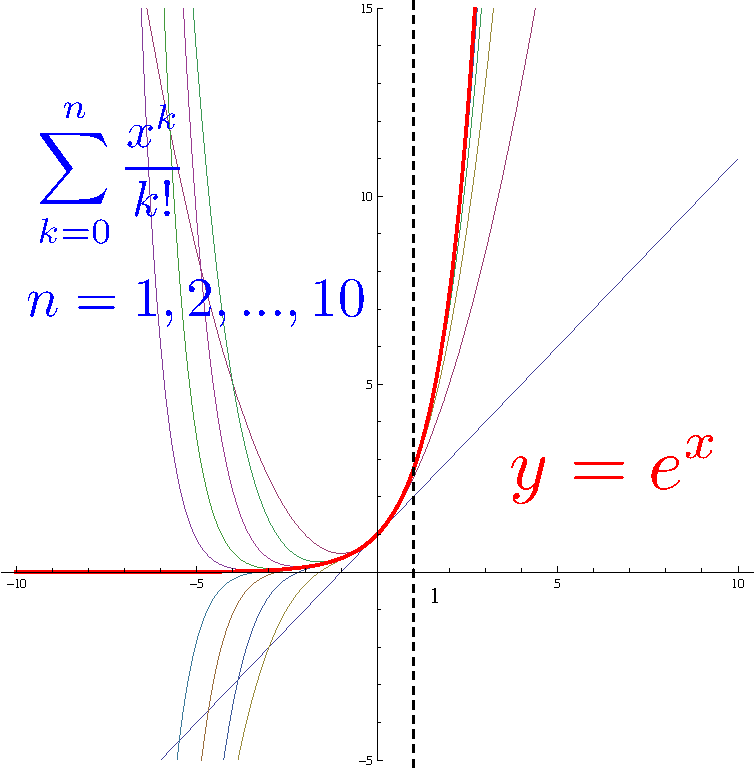
\includegraphics{./images/ch5/exse1.pdf}}
			\end{center}\pause 
		\column{.5\textwidth}
			\begin{center}
				\resizebox{!}{5.5cm}{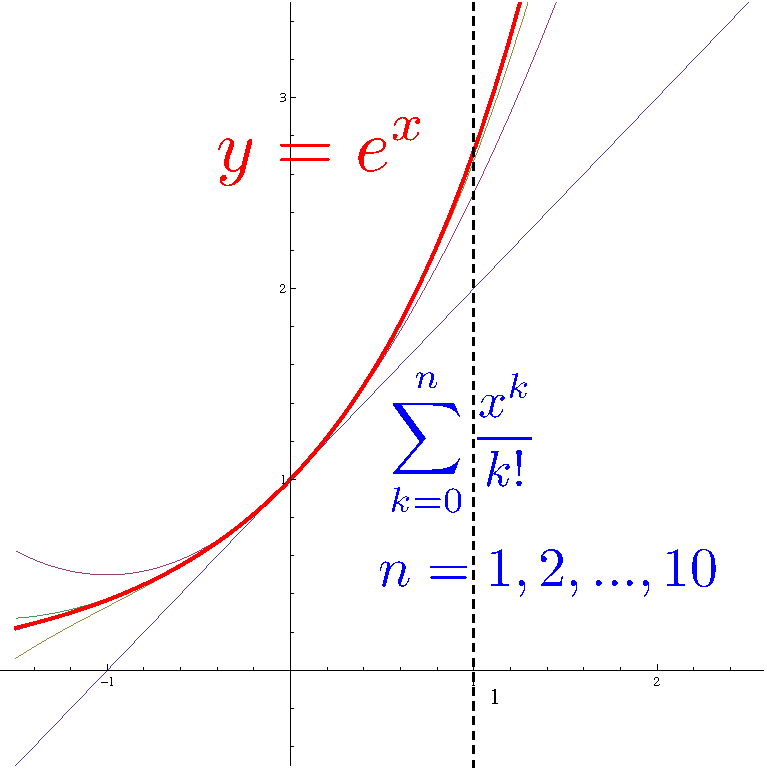
\includegraphics{./images/ch5/exse2.pdf}}
			\end{center}
	\end{columns}
\end{frame}

\begin{frame}{2. 计算不定式极限}
	\linespread{1.2}\pause 
	\begin{exampleblock}{{\bf 例7:}计算以下极限\hfill P257-例8}
		\begin{enumerate}
		  \item $\limx{0}\df{\cos x-e^{-x^2/2}}{x^4}$\pause 
% 		  \item $\limx{0}\df{\tan x-\sin x}{x^3}$\pause 
		  \item $\limx{0}\df{\df{x^2}{2}+1-\sqrt{1+x^2}}{x^2\sin x^2}$\pause 
		  \item $\limx{0}\df{e^x-1-x}{\df{1}{\sqrt{1-x}}-\cos\sqrt x}$\pause 
		\end{enumerate}
% 		\begin{columns}
% 			\column{.41\textwidth}
% 				\begin{enumerate}
% 				  \item $\limx{0}\df{\cos x-e^{-x^2/2}}{x^4}$
% 				  \item $\limx{0}\df{\tan x-\sin x}{x^3}$
% 				\end{enumerate}
% 			\column{.59\textwidth}
% 				\begin{enumerate}
% 				  \addtocounter{enumi}{2}
% 				  \item $\limx{0}\df{\df{x^2}{2}+1-\sqrt{1+x^2}}{x^2\sin x^2}$
% 				  \item $\limx{+\infty}\left[x-x^2\ln\left(1+\df 1x\right)\right]$
% 				\end{enumerate}
% 		\end{columns}
	\end{exampleblock}
	{\bf 注:}\alert{不知道该展开到多少阶时,先进行试探性展开}
\end{frame}

\begin{frame}
	\linespread{1.2}
	\begin{alertblock}{{\bf 例8:}\hfill}
		设$f(x)$在$x=0$附近二次可导,且
		$$\limx{0}\left(1+x+\df{f(x)}{x}\right)^{1/x}=e^3,$$
		求:
		\begin{enumerate}
		  \item $f(0),f\,'(0),f\,''(0)$;
		  \item $\limx{0}\left(1+\df{f(x)}{x}\right)^{1/x}$.
		\end{enumerate}
	\end{alertblock}
\end{frame}

\begin{frame}{3. 证明不等式}
	\linespread{1.2}\pause
	\begin{exampleblock}{{\bf 例9:}\hfill P258-例9}
		证明:$x>0$时,$e^x>1+x+\df{x^2}{2}$
% 		\begin{enumerate}
% 		  \item $x>0$时,$e^x>1+x+\df{x^2}{2}$\pause
% 		  \item $x\ne 0$时,$e^x>1+x+\df{x^2}{2}+\df{x^3}{6}$
% 		\end{enumerate}
	\end{exampleblock}
	\bigskip\pause
	\begin{exampleblock}{{\bf 例10:}\hfill P259-例10}
		设$f(x)$在$(a,+\infty)$内具有二阶导数,且$f(x),f\,''(x)$在$(a,+\infty)$
		有界,证明:$f\,'(x)$在$(a,+\infty)$有界。
	\end{exampleblock}
\end{frame}

\begin{frame}
	\linespread{1.5}
	\begin{alertblock}{{\bf 例11}\hfill }
		设在$f(x)$在$[0,a]$上二阶连续可导,$|f\,''(x)|\leq M$,且$|f(x)|$在$(0,a)$内可取到最大值,证明:
		$$|f\,'(0)+f\,'(a)|\leq Ma.$$
	\end{alertblock}
\end{frame}

\begin{frame}
	\linespread{1.5}
	\begin{alertblock}{{\bf 例12}\hfill }
		设$f(x)$在$[0,1]$上二阶连续可导,且$f(0)=f(1)$, \\
		$|f\,''(x)|\leq A$,
		证明:对任意$x\in[0,1]$,恒有
		$$|f\,'(x)|\leq\df A2.$$
	\end{alertblock}
\end{frame}

\begin{frame}
	\linespread{1.5}
	\begin{alertblock}{{\bf 例13}\hfill 辅导书P153-例37}
		设$f(x)$在$[a,b]$上二阶连续可导,且$f\,'(a)=f\,'(b)=0$,则至少存在一点
		$c\in(a,b)$,使得
		$$|f\,''(c)|\geq \df 4{(b-a)^2}|f(b)-f(a)|.$$
	\end{alertblock}
\end{frame}


\begin{frame}[<+->]{小结}
	\linespread{1.5}
	\begin{enumerate}
	  \item {\bf Taylor多项式}
	  \item {\bf 函数的Taylor展开}
	  \begin{itemize}
	    \item 直接法
	    \item 间接法
	  \end{itemize}
	  \item {\bf Taylor公式的应用}
	  \begin{itemize}
	    \item 计算极限
	    \item 证明不等式
	  \end{itemize}
	\end{enumerate}
% 	\bigskip
% 	\pause
% 	\centerline{\ba{请自行阅读第六章\S 6.3节}}
\end{frame}

\begin{frame}{课堂练习}
	\linespread{2}
	\begin{exampleblock}{{\bf 例14:}计算下列极限\hfill}
		\begin{enumerate}
% 		  \item $\limx{0}\df{e^x-1-x}{\df{1}{\sqrt{1-x}-\cos\sqrt x}}$
		  \item $\limx{0}\df{\cos(\sin x)-\cos x}{x^4}$
		  \item $\limx{+\infty}\left[x-x^2\ln\left(1+\df 1x\right)\right]$
		\end{enumerate}
	\end{exampleblock}
\end{frame}

\begin{frame}{课堂练习}
	\linespread{1.2}
	\begin{exampleblock}{{\bf 例15}\hfill}
		证明:若在$(a,b)$内,$f\,''(x)>0$,则对任意$a<x_1<x_2<b$,恒有
		$$f\left(\df{x_1+x_2}{2}\right)<\df{f(x_1)+f(x_2)}{2}.$$
	\end{exampleblock}\pause 
	{\bf 思考:}以上结论能否进一步推广?\pause 
	$$\alert{f(\lambda x_1+(1-\lambda)x_2)<\lambda
	f(x_1)+(1-\lambda)f(x_2),\;0<\lambda<1}$$
\end{frame}

%===================================

% \begin{frame}{title}
% 	\linespread{1.2}
% 	\begin{block}{{\bf title}\hfill}
% 		123
% 	\end{block}
% \end{frame}